\documentclass[../thesis/thesis.tex]{subfiles}
\renewcommand{\baselinestretch}{1.5}\selectfont
\graphicspath{{../figs/ch4-vnaunc/}}

\begin{document}
	
\onlyinsubfile{\setcounter{chapter}{3}}

\begin{refsection}
\chapter{Evaluating Uncertainty in Vector Network Analyser Measurements}
\section{Introduction}
The dramatic growth of radio-based devices and applications over the last 50 years has led to the VNA becoming a critical instrument in most laboratories. Many of these applications required both accurate and reliable measurements from these VNAs.  This is particularly so in areas such as manufacturing, calibration and testing.  This is often driven by requirements given in international Quality Management documents such as the ISO 9000 series of standards \cite{ISO9000} (for manufacturing and process control) and the ISO 17025 standard \cite{ISO17025} (for calibration and testing).

The requirements given in these international standards are for measurements that can be demonstrated as fit-for-purpose (in terms of the achievable level of accuracy, etc) and made traceable to the international system of units \cite{SI_2019, SI_2019B}.  These requirements are not trivial for a VNA due to the complicated nature of the VNA’s operating principles, for example the calibration mathematics. Combined with the available computing power and cost at that time, a full or rigorous evaluation of uncertainty for VNA measurements was difficult and time-consuming. This led to much work by experts in this field to develop easier methods that addressed these needs in ways that were suitable for use by end-users in the manufacturing, calibration and testing communities.  Much of this work was undertaken by the ANAMET Technology Group (www.npl.co.uk/anamet) during the 1990s.  This resulted in a series of reports \cite{ANAMET_1996, ANAMET_1998, ANAMET_1999} describing the development of a guidance document that gave a procedure for assessing the performance of calibrated VNAs.  The resulting guidance document \cite{EA_2000} was published by the European co-operation for Accreditation (EA, www.european-accreditation.org) so that laboratories operating to the ISO 17025 standard and/or ISO 9000 series of standards could implement the method for their own purposes.  Ownership of this EA document was later transferred to the European Association of National Metrology Institutes (EURAMET) and re-published \cite{EURAMET_2011} as part of their Calibration Guides series of documents. This document, along with the recent updated version, is available as a free download from the EURAMET web-site: www.euramet.org.

In addition to the EURAMET guide, VNA manufacturers have also produced their own advice for users to estimate the combined standard uncertainty in their measurements \cite{Hiebel_2008} and provided software tools in some cases \cite{KeysightUncTool, AnritsuUncTool}. Often this advice is based on the same methods presented in the EURAMET guide, which work by evaluating the residual error in VNA calibrations.

\section{Evaluating Residual Error in VNA Calibrations}

\subsection{Method}

The EURAMET Guide \cite{EURAMET_2011} presents a process for evaluating the uncertainty of measurements performed on a calibrated VNA, allowing users to verify that values measured using the instrument are of acceptable accuracy. This process involves measuring a selection of dominant contributions to measurement uncertainty and combining them appropriately. Contributions include both systematic errors, which remain constant over the period of measurements, and random errors, which do not.  The error model for voltage reflection coefficient (VRC) measurements performed with a VNA is represented in \cite{EURAMET_2011} by the following equations for one-port (1) and two-port (2) measurements:

\begin{align}
U_{\textrm{VRC}} &= D + T\Gamma + M\Gamma^2 + R_{\textrm{VRC}}\\
U_{\textrm{VRC}} &= D + T\Gamma + M\Gamma^2 + R_{\textrm{VRC}} + S_{21}^2\Gamma_L
\end{align}

where $U_{\textrm{VRC}}$ is the combined uncertainty in the measurement, $D$ is the residual directivity, $T$ represents the effect of tracking and nonlinearity, $M$ is the residual test port match (TPM), $\Gamma$ is the measured voltage reflection coefficient, $R_{\textrm{VRC}}$ is the sum of all the random contributions, $S_{21}$ is the nominal attenuation of the device-under-test (DUT), and $\Gamma_L$ is the residual load match. The most significant systematic error contributors to the measurement uncertainty are, in most cases, the directivity and TPM.

To perform a VRC measurement, a VNA must be able to separate reflected and incident voltage waves by their direction of travel and then sample using complex receivers. However, various components in the signal path may cause a portion of the incident wave to leak into the reflected wave receiver without having reached the DUT. This directivity error should ideally be removed by applying correction terms extracted during the VNA calibration. However, as no calibration will be perfect, some residual directivity error will remain (referred to as effective directivity in \cite{EURAMET_2011}). To measure the residual directivity, a matched load can be connected to the test port being assessed. This should theoretically reflect no amount of the incident wave and therefore the only voltage present at the reflected wave receiver should be due to the residual directivity. In practice, the matched load will not be perfectly matched (for the same reason the calibration will never be perfect) so it is likely the residual directivity will typically be either over- or underestimated. An improved method, used in \cite{EURAMET_2011} and widely accepted for use with coaxial measurements, is the ripple extraction technique. This uses a similar principle to measure the residual directivity, but significantly increases the accuracy of the residual error evaluation. An illustration of its method is provided in Figure \ref{ch4_fig_ripple1}.

\begin{figure}
	\centering
	\begin{subfigure}{\textwidth}
		\centering
		\includegraphics[width=0.4\textwidth]{Ripple1.png}
		\caption{When measured on the calibrated VNA, the VRC of a perfect matched load would reveal the true origin ($O_\textrm{T}$) of the plot as offset from the calibrated origin ($O_\textrm{C}$) by the residual directivity ($D$). If a realistic matched load offset by a line section is instead measured, the VRC as measured by the VNA ($\Gamma_\textrm{M}$) will be the sum of the residual directivity and the true VRC ($\Gamma_\textrm{A}$). }
	\end{subfigure}
	\\
	\begin{subfigure}{\textwidth}
		\centering
		\includegraphics[width=0.8\textwidth]{Ripple2.png}
		\caption{As $\Gamma_\textrm{M}$ is measured across a swept frequency range, the electrical length of the line increases causing the phase to sweep also. This rotates $\Gamma_\textrm{T}$, resulting in ripples in the plot of $|\Gamma_\textrm{M}|$ against frequency. The magnitude of the ripples is equal to $2D$. }
	\end{subfigure}
	\\
	\begin{subfigure}{\textwidth}
		\centering
		\includegraphics[width=0.8\textwidth]{Ripple3.png}
		\caption{However, if $\Gamma_\textrm{A} < D$, then the ripple magnitude is now $2\Gamma_\textrm{A}$ instead of $2\Gamma_\textrm{D}$ and the residual directivity as evaluated using the ripple extraction technique would be underestimated.}
	\end{subfigure}
	\caption{An illustration of the ripple technique measuring residual directivity.}
	\label{ch4_fig_ripple1}
\end{figure}

To perform the evaluation, a short length of line is connected to the test port, to the end of which is added a matched load covering the frequency range under test. The line section should be traceable to national standards and have a characteristic impedance identical to that of the VNA setup. For these reasons a beadless airline is suggested in \cite{EURAMET_2011}. The load can be either the same as that used for calibration or another with $0.1 \ge \Gamma \ge 0.2$ to ensure that $\Gamma \ge D$. If $\Gamma < D$, then the measured residual directivity will be underestimated as explained by Figure \ref{ch4_fig_ripple1}. If the calibration matched load is used for the measurement, the small reflection from a second connection and any loss in the airline will cause the VRC to be greater than the residual directivity from the original measurement of the load. Alternatively, because $\Gamma < 0.1$ for the matched load used for calibration, using another load with a known higher $\Gamma$ ensures that there is no underestimate. Once the instrument has been configured, $\Gamma$ is measured and the magnitude plotted against frequency using a linear scale. A ripple should be clearly visible on the trace, from which the residual directivity can be calculated from:

\begin{equation}
D = \frac{\textrm{Maximum Ripple Amplitude}}{2}
\end{equation}

For coaxial measurements as specified in \cite{EURAMET_2011}, there is a high probability that the condition required to avoid underestimation is met. However, in order to assess the suitability of the technique in waveguide a method of assessing this condition has been used. By examining either a complex plot (polar or Smith chart) or a phase plot, the geometric symptom shown in Figure \ref{ch4_fig_ripple1} can be identified. When using a complex plot, the origin should lie within the circumference of the reflection coefficient trace for the residual error to be accurately measured. For any frequency range where it does not, the ripple technique provides an underestimation of the residual error. When using a phase plot, there will be regular wrapping of the reflection coefficient phase for frequency ranges where the residual error is correctly measured, whereas when underestimation occurs the phase will vary by less than 180 degrees per period. An example of both plots are shown in Figure \ref{ch4_fig_dir}. Either of these methods can be used to identify when a calibration and ripple measurement needs to be repeated. If the repeat measurements still fail the test, then the choice of loads may need to be altered.

\begin{figure}
	\centering
	\includegraphics[width=0.36\textwidth]{dir_smith.png}
	\hfill
	\includegraphics[width=0.58\textwidth]{dir_xy.png}
	\caption{Smith chart and phase plot of a residual directivity measurement performed in coaxial transmission line using the calibration load (solid line) and a load from a different calibration kit (dotted line). The intersection of the grid lines on the Smith chart represents the origin of the plot ($\Gamma = 0$). The measurement which used the different load indicate an accurate residual directivity estimate across the entire measured spectrum. The measurement which used the calibration load suggests an underestimate of the residual directivity is likely between 16--22 GHz.}
	\label{ch4_fig_dir}
\end{figure}

TPM is caused by imperfections in the impedance match between components in the VNA setup. This causes delayed reflections that interfere with the DUT measurement and can provide false values. Calibration also corrects for TPM, but as with directivity some residual error will remain. To measure residual TPM, a short circuit is connected to the test port being assessed. This should reflect the entire incident signal and therefore maximise any reflections in the VNA setup. If residual TPM error is present then the measured VRC will be less than 1. However, the short circuit may not provide a perfect reflection and so the ripple extraction technique is favoured for this measurement also.

To measure residual TPM using the ripple extraction technique, the same procedure as for residual directivity is followed but the matched load at the end of the line is replaced by a short circuit. A similar plot is acquired and the residual TPM is given by:

\begin{equation}
M = \frac{\textrm{Maximum Ripple Amplitude}}{2}
\end{equation}

Because the reflection coefficient for this measurement should be close to 1, there is no risk that this value will be greater than the true residual TPM and cause an underestimate as can be the case for residual directivity. This is shown in Figure \ref{ch4_fig_tpm}, where the origin of the Smith chart is clearly inside the circular trace and the phase consistently wraps across the entire measured spectrum.

\begin{figure}
	\centering
	\includegraphics[width=0.36\textwidth]{tpm_smith.png}
	\hfill
	\includegraphics[width=0.58\textwidth]{tpm_xy.png}
	\caption{Smith chart and phase plot of a residual TPM measurement performed in coaxial transmission line using the calibration short circuit (solid line) and a short circuit from a different calibration kit (dotted line). Both measurements indicate an accurate residual TPM estimate across the entire measured spectrum. Residual TPM measurements avoid the risk of underestimation via the mechanism described for residual directivity measurements due to the typical VRC being close to one (far from the origin of the Smith chart).}
	\label{ch4_fig_tpm}
\end{figure}

To perform the technique for both described residual error sources requires just three components: A short circuit, matched load, and a short section of line. These components are realizable in both coaxial and rectangular waveguide, so the technique should be physically possible to perform in waveguide setups. The technique can be applied to any type of calibration – for example three-known-loads and thru-reflect-line (TRL). In coaxial, the short-open-load-thru (SOLT) variant of the former is used. However, in waveguide an open circuit is not straightforward to realise or widely adopted, so a common variant of SOLT calibration which uses an offset short (SOSLT) can be used instead.

\subsection{Investigation of ripple technique effectiveness with waveguide VNA calibrations}

Although both the EURAMET guide and VNAs using rectangular metal waveguide test ports have both existed for many years, there was no published evidence that the methods employed in the guide (the ripple technique) could be successfully applied to those measurements. The author undertook an investigation into this during the degree where they compared residual error measurements in coaxial line to those in waveguides at frequencies ranging from 8.2 GHz to 750 GHz (submillimetre-wave). This section presents the results of the subsequent papers \cite{Stant_2016_Coll, Stant_2017}.

\subsubsection{Coaxial Transmission Line and Microwave Waveguide}

The ripple extraction technique was first performed on coaxial line in accordance with the EURAMET Guide \cite{EURAMET_2011} instruction as described in the previous section. The guide itself provides a range of typical values for both residual directivity and TPM ripple measurements with which our results can be compared to ensure that the process was followed correctly. All measurements presented in this investigation were acquired using a Keysight 5247A PNA-X instrument fitted with 1.85 mm ports attached to flexible port extender cables with rugged connectors. The coaxial measurement setup used a 7.5 cm beadless airline and the calibration kit matched load and short circuit. Figure \ref{ch4_fig_coax_load} shows the ripple trace obtained by plotting VRC magnitude against frequency for a residual directivity measurement on both ports using a SOLT calibration. Figure \ref{ch4_fig_coax_short} shows a similar ripple measured with a short circuit instead of a matched load, which is caused by the residual TPM. The results of the measurements, along with the expected ranges provided in \cite{EURAMET_2011}, are presented in Table \ref{ch4_table_coax}.

\begin{figure}
	\centering
	\includegraphics[width=0.65\textwidth]{coaxial_load.png}
	\caption{Magnitude of the reflection measurement of a matched load offset by a short line length in coaxial media. The VNA was calibrated using the SOLT method, and measurements were performed on both port 1 (solid line) and port 2 (dotted line). Variations apart from the dominant ripple are due to the imperfect response of the matched load and the beadless line.}
	\label{ch4_fig_coax_load}
\end{figure}

\begin{figure}
	\centering
	\includegraphics[width=0.65\textwidth]{coaxial_short.png}
	\caption{Magnitude of the reflection measurement of a short circuit offset by a short line length in coaxial transmission line. The VNA was calibrated using the SOLT method, and measurements were performed on both port 1 (solid line) and port 2 (dotted line). The increasing attenuation with frequency is characteristic of the beadless airline.}
	\label{ch4_fig_coax_short}
\end{figure}

\begin{table}[]
	\begin{tabular}{lllll}
		\hline
		& \begin{tabular}[c]{@{}l@{}}Port 1 \\   Residual Directivity\end{tabular} & \begin{tabular}[c]{@{}l@{}}Port 2\\   Residual Directivity\end{tabular} & \begin{tabular}[c]{@{}l@{}}Port 1\\   Residual TPM\end{tabular} & \begin{tabular}[c]{@{}l@{}}Port 2\\   Residual TPM\end{tabular} \\ \hline
		SOLT            & 0.0075                                                                   & 0.0085                                                                  & 0.0135                                                          & 0.0100                                                          \\
		TRL             & 0.0075                                                                   & 0.0070                                                                  & 0.0015                                                          & 0.0015                                                          \\
		cg-12 Reference & 0.002—0.02                                                               & 0.002—0.02                                                              & 0.005—0.02                                                      & 0.005—0.02                                                      \\ \hline
	\end{tabular}
	\caption{Residual directivity and TPM values of 3.5mm coaxial line VNA calibrations as measured by the ripple extraction method. Both SOLT and TRL calibration techniques were measured.}
	\label{ch4_table_coax}
\end{table}

It can be seen that the measured values for the coaxial line setup fall well within the typical ranges. The same method was applied to two types of centimetre band waveguide, WG16 (WR90) and WG20 (WR42). These waveguides have usable frequency ranges of 8.2—12.4 GHz and 18.0—26.5 GHz respectively. In order to avoid the effects of non-propagating (evanescent) modes created by the waveguide test adapter, a section of standard line with length equal to several times the aperture width was attached to each adapter where possible and the measurement planes defined at the end of the lines. The results of the ripple extraction are shown in Table \ref{ch4_table_WG16}:

\begin{table}[]
	\begin{tabular}{lllll}
		\hline
		& \begin{tabular}[c]{@{}l@{}}Port 1\\ Residual Directivity\end{tabular} & \begin{tabular}[c]{@{}l@{}}Port 2\\ Residual Directivity\end{tabular} & \begin{tabular}[c]{@{}l@{}}Port 1\\ Residual TPM\end{tabular} & \begin{tabular}[c]{@{}l@{}}Port 2\\ Residual TPM\end{tabular} \\ \hline
		WG16 SOSLT & 0.0045                                                                & 0.0040                                                                & 0.0070                                                        & 0.0060                                                        \\
		WG16 TRL   & 0.0030                                                                & 0.0060                                                                & 0.0020                                                        & 0.0015                                                        \\
		WG20 SOSLT & 0.0030                                                                & 0.0040                                                                & 0.0095                                                        & 0.0050                                                        \\
		WG20 TRL   & 0.0020                                                                & 0.0020                                                                & 0.0015                                                        & 0.0010                                                        \\ \hline
	\end{tabular}
	\caption{Residual directivity and TPM values of WG16 and WG20 waveguide VNA calibrations as measured by the ripple extraction method. Both SOSLT and TRL calibration techniques were measured.}
	\label{ch4_table_WG16}
\end{table}

\subsubsection{Millimetre-wave Waveguides}

To perform measurements above the 67 GHz upper limit of the VNA used for the investigation, a range of VDI frequency extender heads were attached to the instrument. These instruments include on their test port a line section of suitable length to allow the dissipation of evanescent modes. To study the performance of the ripple extraction technique at millimetre wavelengths, WG25 (WR15) and WG30 (WR05) waveguides were chosen. These waveguides have operating frequency ranges of 50—75 GHz and 140—220 GHz respectively. The results of the ripple extraction are shown in Table \ref{ch4_table_WG25}:

\begin{table}[]
	\begin{tabular}{lllll}
		\hline
		& \begin{tabular}[c]{@{}l@{}}Port 1\\ Residual Directivity\end{tabular} & \begin{tabular}[c]{@{}l@{}}Port 2\\ Residual Directivity\end{tabular} & \begin{tabular}[c]{@{}l@{}}Port 1\\ Residual TPM\end{tabular} & \begin{tabular}[c]{@{}l@{}}Port 2\\ Residual TPM\end{tabular} \\ \hline
		WG25 SOSLT & 0.0015                                                                & 0.0015                                                                & 0.0175                                                        & 0.0165                                                        \\
		WG25 TRL   & 0.0015                                                                & 0.0020                                                                & 0.0090                                                        & 0.0070                                                        \\
		WG30 SOSLT & 0.0075                                                                & 0.0090                                                                & 0.0185                                                        & 0.0235                                                        \\
		WG30 TRL   & 0.0070                                                                & 0.0080                                                                & 0.0210                                                        & 0.0150                                                        \\ \hline
	\end{tabular}
	\caption{Residual directivity and TPM values of WG25 and WG30 waveguide VNA calibrations as measured by the ripple extraction method. Both SOSLT and TRL calibration techniques were measured.}
	\label{ch4_table_WG25}
\end{table}

\subsubsection{Submillimetre-wave Waveguides}

The final part of the investigation studied the ripple extraction technique when applied to sub-millimetre wavelength VNA setups. The waveguide chosen for these measurements was in the 500—750 GHz band (WR1.5) for which only one frequency extender head was available. Therefore, the TRL calibration was omitted and only port one was measured. The line section used was part of the VDI WR1.5 calibration and verification kit and was 2.54 mm (1 inch) in length. Figure \ref{ch4_fig_setup} shows the setup used during the measurement of residual directivity, with a line and match connected to the frequency extender head. The results from the ripple measurements in this waveguide are presented in Table \ref{ch4_table_WR1.5}. The large difference in residual TPM error between calibrations suggests that there is poor connection repeatability between the waveguide components, an issue which is explored further in the following section. This problem also created difficulty in accurately measuring the residual directivity error, as studying the VRC phase revealed that there was no wrapping present and on average only ~90 degree total phase deviation. Figure \ref{ch4_fig_wm380} shows the result of this measurement, which suggests that the residual directivity will be underestimated using the ripple extraction technique with this data. The calibration kit included two sets of standards, so the load was swapped but did not improve the problem. Rotation of the load about 180 degrees, which is possible with the UG-387 flange design, also did not increase the phase deviation. The same issue was found when the measurements were performed using the second calibration, which used the entire second set of calibration standards in the kit. This behaviour suggests that the connection repeatability issue is also likely to blame for the residual directivity underestimation. If the matched load was connected with a flange misalignment that caused more reflection than when the line was subsequently added, then $\Gamma < D$ and the ripple technique will fail.

\begin{figure}
	\centering
	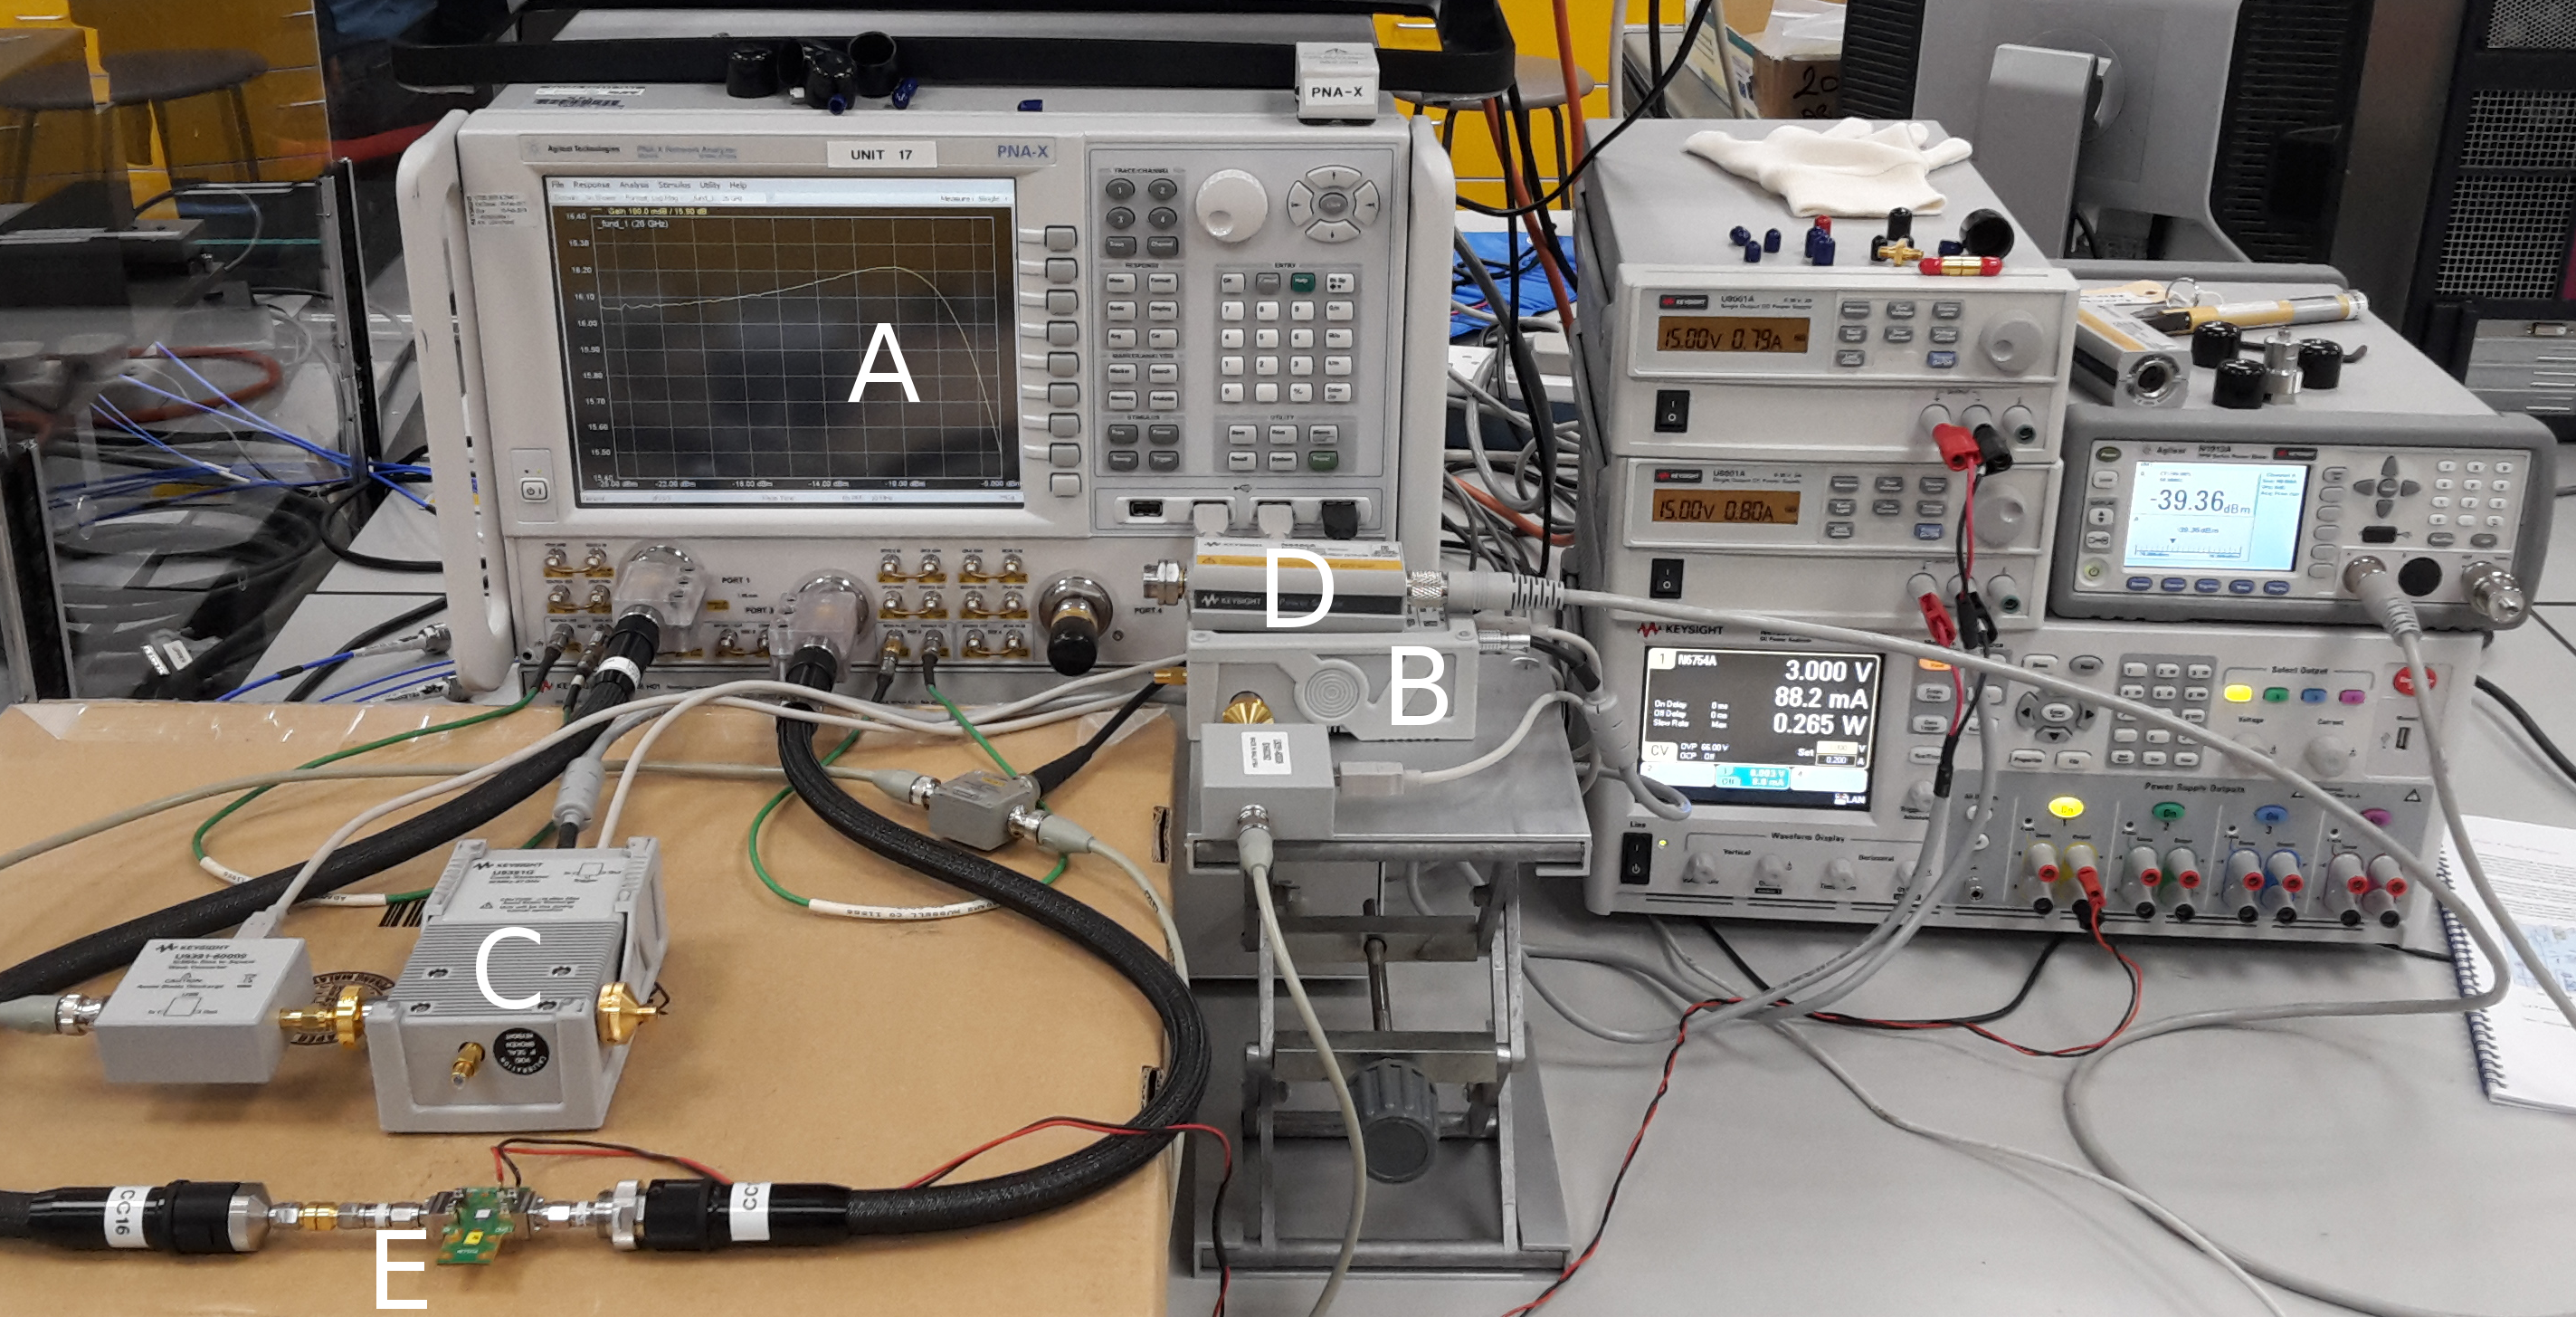
\includegraphics[width=0.65\textwidth]{setup.jpg}
	\caption{The setup used for residual directivity measurements in WR1.5 waveguide.}
	\label{ch4_fig_setup}
\end{figure}

\begin{table}[]
	\begin{tabular}{lll}
		\hline
		& \begin{tabular}[c]{@{}l@{}}Port 1\\ Residual Directivity\end{tabular} & \begin{tabular}[c]{@{}l@{}}Port 1\\ Residual TPM\end{tabular} \\ \hline
		WR1.5 SOSLT Cal. 1 & 0.0205                                                                & 0.1420                                                        \\
		WR1.5 SOSLT Cal. 2 & 0.0250                                                                & 0.0650                                                        \\ \hline
	\end{tabular}
	\caption{Residual directivity and TPM values of two WR1.5 waveguide VNA calibrations as measured by the ripple extraction method. Two similar calibrations were performed using different standards from the same kit.}
	\label{ch4_table_WR1.5}
\end{table}

\begin{figure}
	\centering
	\includegraphics[width=0.65\textwidth]{wm380.png}
	\caption{Phase plot for a residual directivity measurement performed in WR1.5 waveguide using a SOLT calibration. The lack of phase wrapping over the entire operating bandwidth indicates that the ripple extraction technique will underestimate the residual error.}
	\label{ch4_fig_wm380}
\end{figure}

\subsubsection{Waveguide Discontinuities}

When a discontinuity is present between two sections of rectangular waveguide, an increased reflection will be seen at the location of the join. There are three types of discontinuity possible in rectangular waveguide: E-plane and H-plane lateral displacements, angular displacement, and corner rounding. A report produced by Bannister \cite{Bannister_1989} presented the effects of these discontinuities at centimetre and millimetre wavelengths with measured data, and subsequent work by Kerr extended this using simulations \cite{Kerr_1999, Kerr_2010}. 

The error in VRC contributed to by this effect is proportional to wavelength and therefore the aperture size of the waveguide. At submillimetre wavelengths, the error has been shown to be considerable \cite{Williams_2011, Li_2012}. Recently, efforts have been made to improve the connection repeatability for waveguide at these wavelengths, and a new IEEE draft standard \cite{IEEE1785} presents three new connector types which significantly improves the alignment. Another potential improvement attempts to reduce misalignment errors during calibration by replacing the waveguide offset short with a radiating open, and new calibration algorithms have been developed to accompany this \cite{Arsenovic_2014}. The open standard must be very well characterised, and the technique has not yet seen widespread uptake.

\subsubsection{Discussion}

In centimetre wavelength band waveguides (WG16, WG20) the ripple extraction technique provided similar measurements of residual directivity and TPM than those performed in coaxial line. This is not surprising as providing a good quality match was used for calibration and the connections were well made and aligned, both errors should not have significant contributions outside of the VNA itself. When extended to millimetre wavelength waveguide, the residual errors were larger but still within the recommended values for coaxial lines. At sub-millimetre wavelengths the two calibrations resulted in significant differences in the residual error. A likely cause is the effect of discontinuities in the waveguide components during calibration, especially the matched load and offset short. Additionally, by studying the phase of the measured VRC, it was shown that the residual directivity measurements were underestimating the true value and therefore the ripple technique was failing. This may also be due to the poor repeatability of the waveguide connection causing the VRC of the matched load used for the ripple extraction to be lower than that used for the calibration. Steps were taken to attempt to resolve this issue, but the extent of the misalignment errors prevented an accurate measurement of residual directivity from being performed. New improvements to sub-millimetre wavelength waveguide flanges should significantly reduce this problem and allow the ripple technique to work more consistently with these waveguides.

A useful assessment method for the ripple technique was presented earlier in this section and should be performed whenever the technique is used. When viewing the measured VRC on a polar or Smith chart, if the origin of the chart lies within the circumference of the trace, the technique is accurately measuring the residual error. However, if the trace is circling outside of the origin of the chart, the ripple half-height only represents the magnitude of the reflection measurement used for the technique. If the technique has been deemed failed by this assessment, the VNA should be recalibrated and the test attempted again. If it fails after this, then the test artefacts should be connected in a way that exaggerates the mismatch, for example by inverting a connection, and the test performed again. Only when the origin of the Smith chart lies within the reflection trace are the results from the technique accurate.

\subsubsection{Conclusion}

The investigation studied the effectiveness of the ripple extraction technique when applied to rectangular waveguide measurements up to 750 GHz. Typical values of residual directivity and test port match were provided for users to compare against. The effect of discontinuities at waveguide interconnections were explored and some recent efforts to mitigate these problems were mentioned. Finally, the investigation showed that the ripple extraction technique may not currently be a reliable way of measuring residual error in sub-millimetre wavelength systems.


\section{Sources of VNA Measurement Uncertainty}
\subsection{Calibration Standards}
\subsection{Sources of Random Error}
\subsection{Additional Sources}
\section{Software Frameworks for VNA Uncertainty Evaluation}
\subsection{Standalone Vendor Tools}
\subsection{Keysight PNA-X Dynamic S-Parameter Uncertainty Option}
\subsection{METAS VNA Tools II}
\subsection{NIST Microwave Uncertainty Framework}
\section{Sources of MHVNA Measurement Uncertainty}
\subsection{Power Calibration}
\subsection{Phase References}
\section{Evaluation of Uncertainty in MHVNA Measurements}
\subsection{Measurement Models}
\subsection{Input Quantities}
\subsection{Processing Structure}
\subsection{Results}
\section{Conclusions}

\section{Introduction}
\section{VNA Measurement Model Input Quantities}
\subsection{Calibration Standards}
\subsubsection{Definitions}
\subsubsection{Measurements}
\subsection{Noise}
\subsubsection{Noise Floor}
\subsubsection{Trace Noise}
\subsection{Repeatability}
\subsubsection{Connections}
\subsubsection{Cables}
\subsection{Drift}
\section{Residual Calibration Error VNA Uncertainty Evaluation}
\subsection{Method}
\subsection{Application to Waveguide VNAs}
\section{Rigorous VNA Uncertainty Evaluation}
\subsection{Method}
\subsection{Software Frameworks}
\subsubsection{Keysight PNA-X Dynamic S-Parameter Uncertainty Option}
\subsubsection{METAS VNA Tools II}
\subsubsection{NIST Microwave Uncertainty Framework}
\section{NVNA Uncertainty Evaluation}
\subsection{Phase Reference}
\subsection{Power Meter}
\subsection{Uncertainty Evaluation using MUF}
\section{Conclusion}
\addcontentsline{toc}{section}{Bibliography}
\printbibliography[title=References]
\end{refsection}
\end{document}
